\chapter{Cell Membranes: A Thinking Boundary?}

\begin{kaichang}
Think about washing your hands. During the pandemic years, you were surely told: use soap and scrub for a full 20 seconds. Curiously, the instructions often called not for ``disinfectant,'' but for ordinary soap. Why soap in particular? Stranger still, doctors will tell you that soap and 75\% alcohol work very well against some viruses but only moderately well against others. They are all viruses, so why the different treatment?

Now look in your kitchen: cut a piece of beetroot and soak it in cold water, and the water barely changes color; put it in hot water, and within minutes the water turns purplish red. The pigments had been safely confined inside cells. What did the hot water do to release them all?

At the end of Chapter 25, we left a question hanging: an egg membrane is semipermeable, letting water through while restricting solutes. A living cell's membrane is far more sophisticated: it comes equipped with ``pumps'' and ``gates.'' This chapter delivers on that promise. First, take a guess: how can a membrane just \textbf{two molecules thick} hold back a vast crowd, admit particular molecules precisely, and even help generate electrical signals in nerves? Is it a boundary that can think?
\end{kaichang}

\section{Phenomena: An Invisible Boundary, Visible Consequences}

You have never seen a cell membrane. Under an ordinary light microscope, it is only a faint outline around a cell, because it is about 4 to 5 nanometers thick, whereas the resolution limit of a light microscope is about 200 nanometers. More than ten thousand cell membranes could fit side by side across the diameter of a hair.

Yet the consequences of this invisible boundary are everywhere:

\begin{itemize}[itemsep=2pt]
\item Place red blood cells in pure water, and they absorb water and burst. Bright red hemoglobin leaks out, and the suspension becomes transparent. This is the osmotic pressure calculated in Chapter 25 at work: water molecules flow into the cells on balance from the pure-water side, and the membrane can withstand only limited expansion.
\item Place red blood cells in concentrated salt water, and they lose water and shrivel like dried raisins. Only in 0.9\% physiological saline do they remain unharmed: isotonic, neither too much nor too little.
\item The glucose you eat appears in your blood within minutes to hours and is rapidly taken up by cells throughout your body. Glucose molecules are much larger than water molecules and cannot cross an ordinary lipid membrane, yet cells can keep transporting them inside.
\item Touch a scalding cup, and your fingers withdraw almost instantly. The signal races along nerves at tens of meters per second. Its essence is wave after wave of charged ions rushing across nerve-cell membranes.
\end{itemize}

It lets water through, blocks sugar yet admits it, and even generates electricity: this boundary has a far more complex character than an egg membrane. To understand it, we must zoom down to the molecular scale and see what the membrane is made of.

\section{Particles: Phospholipids That Line Up by Themselves}

You met the membrane's main building material in Chapter 47: phospholipids. Each has a water-loving ``head'' containing a phosphate group and two water-avoiding ``tails,'' long fatty-acid chains. As we noted then, this split personality makes phospholipids assemble spontaneously into a bilayer in water: tails face tails inside, away from water, while the heads face the water on both outer surfaces. No blueprint, no foreman: just self-assembly driven by the hydrophobic effect.

Now pause to appreciate how remarkable this is. Scatter phospholipids into water, and they form hollow spheres \textbf{by themselves}, enclosing little pools of water and separating them from their surroundings. In other words, \textbf{the boundary emerges from the molecules themselves}. This is anything but trivial. Chapter 45 named ``having a boundary'' as the first feature of a living system. Only a boundary creates an ``inside'' and an ``outside,'' allowing a cell to maintain an internal environment different from its surroundings. The phospholipid bilayer supplies just such a boundary: it allows water and a few small molecules through while excluding most ions, sugars, and amino acids, or at least making their passage extremely difficult.

How thin is it? The entire bilayer is about 4 to 5 nanometers thick, the length of two phospholipid molecules placed end to end. An order-of-magnitude estimate gives a feel for both ``thin'' and ``many.'' A red blood cell is roughly a disk indented on both sides, with a surface area of about 140 square micrometers, or $1.4\times 10^{-10}$ square meters. One phospholipid head occupies about $0.7$ square nanometers, or $0.7\times 10^{-18}$ square meters. Since the membrane has two layers, with an inner and an outer surface, its total number of phospholipid molecules is about

\[2\times \frac{1.4\times 10^{-10}}{0.7\times 10^{-18}} = 4\times 10^{8}\]

It takes about \textbf{400 million phospholipid molecules} to cover one tiny red blood cell. Your whole body contains more than 20 trillion cells. Although membranes are too thin for a light microscope to resolve, building them is an undertaking of astonishing scale.

Remember another detail: a membrane is not a uniform sheet of phospholipids. It contains many embedded proteins; in some membranes, proteins outweigh lipids. Cholesterol is scattered among them, acting, as Chapter 47 noted, like a ``consistency adjuster'' that maintains suitable fluidity at different temperatures. Sugar chains hang from the outer surface: Chapter 46 described them as the cell's ``identity tags,'' recognized by other cells. This is a wall built from several materials, and it is constantly flowing.

``Constantly flowing'' is not a figure of speech but a functional necessity. If the membrane is too stiff, embedded proteins cannot move, change shape, or work; if it is too fluid, it cannot retain what should stay inside. Organisms actively adjust its consistency. Cold-tolerant fish and overwintering plants increase the proportion of unsaturated fatty acids in their membrane lipids. Recall Chapter 47: unsaturated chains have bends and cannot pack tightly. Like antifreeze mixed into oil, they keep the membrane flexible at low temperatures. Your cells use cholesterol for a similar purpose. Fever and frostbite damage cells partly because temperature pushes membrane fluidity outside its normal range.

\section{Rules: What Crosses, and How?}

Now for the central issue: the membrane's traffic rules. Ultimately, substances cross cell membranes by just three routes, distinguished by two questions: \textbf{Is protein assistance needed?} and \textbf{Is energy consumed?}

\textbf{Route one: simple diffusion.} Small molecules squeeze directly through gaps in the phospholipid bilayer without help. Oxygen, carbon dioxide, and most water take this route. The direction is always from higher to lower concentration, downhill along the gradient. This is the same statistical rule behind diffusion and osmosis in Chapter 25: nobody directs the traffic; more molecules simply collide their way across from the more concentrated side. Osmosis is really the simple diffusion of water across a membrane. Chapter 25 examined it thoroughly, so we will not repeat that discussion.

\textbf{Route two: facilitated diffusion.} Glucose and various ions want to cross, but the bilayer's hydrophobic interior does not welcome them: sugars are too hydrophilic, and ions carry charge. They need dedicated routes built from membrane proteins: glucose transporters for glucose, aquaporins for water, and distinct ion channels for different ions. Notice that although this route requires a helper, it \textbf{does not consume energy}; movement is still downhill along a gradient. The protein merely lowers the barrier to crossing. In Chapter 49's language, it lowers the ``activation energy'' without changing the direction. The concentration gradient determines the direction, and nobody can change it.

\textbf{Route three: active transport.} This is the truly forceful route: pumping substances uphill against a gradient, from lower to higher concentration. Going uphill requires energy, supplied by coupling ATP hydrolysis to transport, as discussed in Chapter 50. The best-known example is the sodium--potassium pump. For every ATP it hydrolyzes, it pumps 3 sodium ions out of the cell and 2 potassium ions in. Both movements are against their concentration gradients.

Why go to all this trouble? Because a gradient is itself a resource. Sodium is more abundant outside cells and potassium inside, an asymmetry that the sodium--potassium pump pays ATP to maintain continuously. The return on that investment is immediate: whenever needed, opening a channel lets ions rush downhill and releases an electric current. It is like pumping water into an elevated storage tank, then opening a tap when you need running water. The gradient is the cell's deposit of potential energy.

All three routes operate around you day and night. Kidney-tubule cells use aquaporins to recover water rapidly: roughly 180 liters of initial filtrate are produced daily, but reabsorption leaves only a liter or two of urine. Some diuretics interfere with ion reabsorption in the tubules, preventing water from being retained. Blocking channels, meanwhile, can cause poisoning. Tetrodotoxin fits into the openings of sodium channels in nerve cells, halting the ion flood and paralyzing nerve signals. That is why preparing pufferfish requires a license: this is not mysticism but a life-or-death matter of membrane-protein geometry.

\textbf{Translator safety note:} The source's licensing remark is not assurance that pufferfish is safe to prepare or eat. Do not prepare it yourself; cooking and freezing do not destroy its toxin. See the \href{https://www.accessdata.fda.gov/cms_ia/importalert_37.html}{FDA pufferfish warning}.

These routes are not isolated. Picture a relay in the small intestine. Glucose concentration is lower in the intestinal lumen than inside a cell, so direct diffusion would be uphill. What now? The cell first uses its sodium--potassium pump to move sodium uphill and out, consuming ATP. A cotransporter then lets sodium flow back downhill, but with a strict rule: sodium must bring glucose through the gate with it. The potential energy released by sodium moving downhill pays for glucose moving uphill. Glucose completes active transport without consuming ATP itself; the sodium--potassium pump actually settles the bill. Every membrane machine follows the same overall accounting rule: energy cannot appear from nowhere, only be passed from one gradient to another.

\begin{qiaoliang}
How large is this deposit? Across nerve- and muscle-cell membranes, sodium concentrations differ by about a factor of 10 and potassium concentrations by about 30. Together with the membrane's much greater permeability to potassium than sodium, this maintains a voltage difference of about $-70$ millivolts, negative inside and positive outside, called the \textbf{membrane potential}. That sounds tiny, but the membrane is only about 5 nanometers thick. Divide voltage by thickness, and the electric field inside the membrane exceeds ten million volts per meter, several times the field around high-voltage transmission lines. Only the tiny distance and therefore small total energy keep it from giving you an electric shock. When sodium channels open, sodium rushes downhill into the cell, and the local potential flips from $-70$ to $+30$ millivolts within a thousandth of a second. This electrical nerve pulse is an action potential. How fast you withdraw your hand depends on how fast this ``ion flood'' travels along the nerve.
\end{qiaoliang}

\section{Symbols: A Map of the Membrane}

Let us compress all this into a diagram. Biologists conventionally use notation such as $[\chem{Na^+}]_{\text{outside}}$ for ``sodium-ion concentration outside the cell,'' arrows for transport directions, and $-70$ mV for membrane potential. The sketch below combines the three transport routes:

\begin{center}
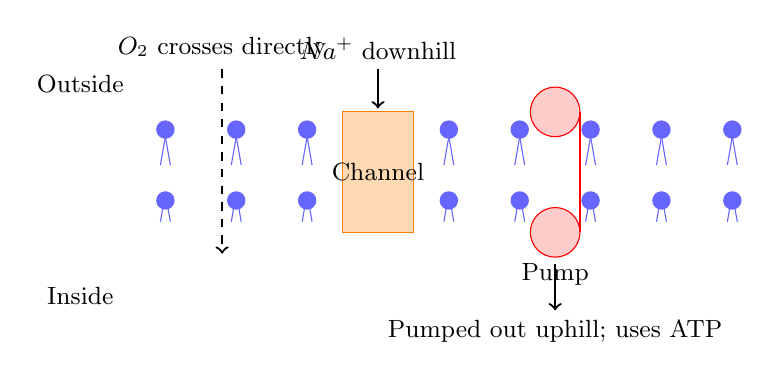
\begin{tikzpicture}[scale=0.9]
\foreach \x in {0,1,2,3,4,5,6,7,8} {
  \fill[blue!60] (\x,0.45) circle (0.13);
  \draw[blue!60] (\x,0.35) -- (\x-0.07,-0.05);
  \draw[blue!60] (\x,0.35) -- (\x+0.07,-0.05);
  \fill[blue!60] (\x,-0.55) circle (0.13);
  \draw[blue!60] (\x,-0.45) -- (\x-0.07,-0.85);
  \draw[blue!60] (\x,-0.45) -- (\x+0.07,-0.85);
}
\draw[orange,fill=orange!30] (2.5,0.7) rectangle (3.5,-1.0);
\node at (3,-0.15) {\small Channel};
\draw[red,fill=red!20] (5.5,0.7) circle (0.35);
\draw[red,fill=red!20] (5.5,-1.0) circle (0.35);
\draw[red,thick] (5.85,0.7) -- (5.85,-1.0);
\node at (5.5,-1.6) {\small Pump};
\draw[->,thick] (3,1.3) node[above]{\small $\chem{Na^+}$ downhill} -- (3,0.75);
\draw[->,thick] (5.5,-1.45) -- (5.5,-2.1) node[below]{\small Pumped out uphill; uses ATP};
\draw[->,thick,dashed] (0.8,1.3) node[above]{\small $\chem{O_2}$ crosses directly} -- (0.8,-1.3);
\node at (-1.2,1.1) {\small Outside};
\node at (-1.2,-1.9) {\small Inside};
\end{tikzpicture}
\end{center}

The usual reminder applies: this is a human representation. Balls and short lines are not photographs of phospholipids. Real molecules have no colors and constantly jostle and exchange positions. The relative sizes of proteins and lipids are also severely compressed: many membrane proteins are taller than the bilayer itself, protruding from both sides like icebergs.

\section{Evidence: Inferring an Unseen Structure}

\begin{zhengju}
For more than half a century, cell membranes were too thin for any microscope to see. How, then, could scientists conclude that they were phospholipid bilayers? The answer is a linked chain of reasoning, complete with wrong turns.

The first step came in 1925. Two Dutch scientists, Gorter and Grendel, devised a clever experiment. They extracted all the lipids from red blood cells, chosen because they lack internal organelles, so nearly all their lipids come from the outer membrane: tidy bookkeeping. They spread the lipids on water as a monomolecular film and measured its total area. The result was exactly \textbf{twice} the red cells' surface area. The conclusion was almost inescapable: cell membranes contain \textbf{two layers} of lipid molecules. An invisible structure had been discovered by counting area. Interestingly, researchers later found two compensating errors in the experiment: lipid extraction was incomplete, and the cell surface area was underestimated. The conclusion was right almost by accident. Scientific history is not always a straight, triumphant path.

The second step took a wrong turn. In 1935, Davson and Danielli proposed that each side of the bilayer was covered by a protein layer, like a sandwich. This ``sandwich model'' dominated textbooks for more than thirty years. Cracks gradually appeared. Electron microscopy did show a three-layer dark structure, apparently supporting the sandwich. Yet if proteins completely covered the lipids, the membrane surface should have uniform chemical properties, which measurements did not show. Worse, many membrane proteins have large hydrophobic regions that could not comfortably lie on its surface.

In 1972, Singer and Nicolson proposed the \textbf{fluid mosaic model}. Proteins are not lids spread over the surface; they are \textbf{embedded} like icebergs in a sea of lipids, some spanning the whole bilayer and others only halfway in. Both lipids and proteins can drift laterally in the membrane plane. One key piece of evidence came from freeze-etching: when a frozen membrane is split, the fracture often runs through the bilayer's middle, exposing a face studded with particles. These are internal faces of membrane-spanning proteins. The sandwich model predicted a smooth face; the evidence condemned it.

The story did not end there. Later research showed that the membrane is not a uniform sea. Cholesterol and certain lipids cluster into relatively stable islands, called lipid rafts, where particular proteins gather. Nor is the membrane a freely flowing surface: fibers of the cell's internal skeleton tether many proteins and restrict their drift. The fluid mosaic model remains the best framework, but it is no longer quite its 1972 version. This is the familiar rhythm of an evidence story: a bilayer inferred from measurements, an overturned sandwich, an established fluid mosaic, and modifications for lipid rafts. At every step, people ask questions, experiment, and seek alternative explanations.
\end{zhengju}

\section{Selective Responses: Judgment Without Awareness}

We can now answer the title's question directly. Cell membranes behave remarkably ``intelligently.'' Glucose arrives and its transporter admits it, while other, similarly structured sugars cannot enter. A neurotransmitter drifts by, activates a particular receptor, and triggers an immediate response. A hormone arrives and is recognized despite a crowd of ignored bystander molecules. It all resembles a discerning gatekeeper.

But remember this book's refrain: do not ask what particles ``want'' to do; ask which route is physically possible. The membrane's judgment comes entirely from three things with no awareness at all:

\begin{itemize}[itemsep=2pt]
\item \textbf{Matching shapes and charges.} The binding sites of transporters and receptors have particular geometries and charge distributions, so only complementary molecules fit. This is the same principle as structure determining protein function in Chapter 48 and induced fit in Chapter 49. It is not recognition but a fit.
\item \textbf{Energy coupling.} Each uphill step in active transport is paid for by ATP hydrolysis or an existing ion gradient. Without an energy input, the pump stops immediately; it has no will to keep working.
\item \textbf{Statistical rules.} The net direction of diffusion and osmosis comes purely from the difference in collision counts on the two sides. No information passes between them; water molecules do not know the concentration opposite them.
\end{itemize}

Receptors make the point especially clearly. Your nose contains hundreds of kinds of olfactory receptors, each with a differently shaped binding pocket that fits different odor molecules. Binding changes a receptor's shape and triggers a chain of molecular events inside the cell, eventually opening ion channels and changing membrane potential: you smell coffee. Not one step involves awareness; it is all shape, energy, and probability. So the answer is that a cell membrane \textbf{does not think}. Its choices follow inevitably from molecular structures and physical laws, just as a lock does not know its key: the shapes simply match. Layering a whole collection of these mechanisms together produces apparently intelligent behavior. This theme---simple rules combining into complex behavior---will echo repeatedly later in the book.

\begin{wuqu}
``A cell membrane is like an intelligent security guard that knows what should enter.'' Counterexamples abound. Carbon monoxide is somewhat similar in shape to oxygen, so hemoglobin is fooled into binding it: the molecular basis of carbon-monoxide poisoning in Chapter 15. The toxin ouabain fits a particular site on the sodium--potassium pump, blocking it and killing the cell as its gradients collapse. Lead ions slip through certain calcium channels because their charges match and their sizes are similar. A genuinely intelligent guard would make none of these fatal mistakes. Membrane recognition is only a game of matching shapes and charges; the consequences of mistaken matches are the entire subject of toxicology. For the same reason, a central strategy in drug design is to make molecules with slightly different shapes that fool, block, or hijack these undiscerning gatekeepers.
\end{wuqu}

\section{Limits: Where the Model Leaks}

The fluid mosaic model is useful, but its boundaries must be stated before use:

\begin{itemize}[itemsep=2pt]
\item ``The membrane is a uniform two-dimensional fluid'' is only an approximation. Lipid rafts, cytoskeletal anchors, and protein clusters make a real membrane more like a city with districts and mooring posts than a uniform soup. The actual motion of membrane proteins remains an active research frontier.
\item ``Channels are always open'' is wrong. Most ion channels have gates controlled by voltage, ligands, or mechanical forces. Half the secret of nerve signaling lies in channels, and the other half in the rules governing their gates. Imagining a channel as a fixed pipe misses the most fascinating part.
\item An artificial phospholipid bilayer is far from a real cell membrane. Real membranes contain hundreds or thousands of lipid species, have asymmetric sides with different lipid compositions maintained at an energy cost, and are densely crowded with proteins. A clean laboratory model membrane is a simplification, not a portrait.
\item Quantitative conclusions such as the osmotic-pressure formula and ``gradients determine direction'' come from the dilute-solution approximation already stated in Chapter 25. Cytoplasm is a crowded, concentrated solution, where everything is only approximately true in a qualitative sense.
\end{itemize}

\begin{shiyan}
\textbf{How Hot Water Dismantles a Cell's Wall}

Materials: a small piece of beetroot or a purple-cabbage leaf, two transparent cups, cold water, hot water at about $60\,^{\circ}\mathrm{C}$ (a water dispenser's hot setting will do), and a paring knife; ask a parent to do the cutting.

\textbf{Translator safety note:} Water at this temperature can cause serious burns within seconds, and dispenser settings do not guarantee $60\,^{\circ}\mathrm{C}$. An adult must measure and handle the hot water and do the cutting; do not test temperature with your skin. See \href{https://www.cpsc.gov/s3fs-public/5098.pdf}{CPSC scald-prevention guidance}.

Procedure: cut two similarly sized pieces of beetroot and gently rinse away pigment leaking from the cut surfaces under tap water. Put one in cold water and the other in hot water. Leave them for 10 minutes without stirring.

Observations: which cup changes color first? How different are the color intensities? Compare them: what happened in the hot water?

Explanation: beetroot's red pigment is normally confined in cell vacuoles, securely enclosed by two lipid bilayers, the vacuolar membrane and cell membrane. Heating makes the bilayers excessively fluid and denatures membrane proteins, as discussed in Chapter 48. Holes appear in the wall, and pigment pours out. The color you see is the membrane's death notice.

Safety: avoid hot-water burns and use heat-resistant cups. The materials have contacted unboiled water and knives; do not eat them afterward.
\end{shiyan}

\section{Back to the Opening: Soap Takes Down a Wall}

We can now answer the handwashing question. Many viruses, including the coronavirus responsible for COVID-19, influenza viruses, and HIV, wear an outer \textbf{envelope}. This is a phospholipid bilayer stolen from a host-cell membrane, with the virus's own proteins inserted. The coat is essential: it both protects the virus and provides docking equipment for invading the next cell. The envelope first fuses with the cell membrane, allowing the viral contents to enter.

What is a soap molecule? A relative of a phospholipid, with a hydrophilic head and a hydrophobic tail, but only one tail. As soap molecules converge on the viral envelope, their tails insert into the bilayer while their heads face outward. This disrupts the balance of self-assembly: the once tightly sealed wall breaks into fragments mixed with soap, the virus's contents leak out, and it is finished. Soap does to a virus more precisely what hot water did in your beetroot experiment. The principle of 75\% alcohol is similar: it dissolves lipids and denatures proteins at the same time. Why not pure alcohol? Pure alcohol instantly coagulates proteins at the surface, effectively welding a protective shell around the virus; with water present, the 75\% formulation best combines penetration and denaturation. Dosage and proportions: chemistry again.

But remember the qualification: not equally effective against every virus. \textbf{Non-enveloped viruses}, including norovirus, poliovirus, and adenoviruses, have shells assembled directly from proteins, with no lipid bilayer to dismantle. Soap is much less effective at killing them; handwashing mainly removes them physically with flowing water. Alcohol also often falls short, and chlorine-containing disinfectants---Chapter 17's temperamental chlorine---are more reliable against them. The claim that alcohol and soap kill every virus fails because it never asks what coat a virus wears. Once again, understanding structure lets us predict whether a method will work: a practical application of the book's recurring question, ``What is it made of, and how is it connected?''

\textbf{Translator safety note:} The discussion of chlorine disinfectants concerns suitable surfaces, not hands: never use household bleach on skin or mix cleaning products. Wash hands with soap and water for at least 20 seconds; hand sanitizer alone does not work well against norovirus. Follow product labels and \href{https://www.cdc.gov/norovirus/prevention/index.html}{CDC norovirus-prevention guidance}.

\section{Going Deeper: Liposomes and What Comes Next}

Membrane principles do more than explain life; engineers now use them in reverse. If phospholipids spontaneously form spheres in water, why not load drugs inside? These carriers are \textbf{liposomes}. Their membranes have the same material as cell membranes and can fuse with them, delivering enclosed drugs directly into cells. Some anticancer drugs are delivered this way. You have probably received an even more famous application: mRNA vaccines package their mRNA in lipid nanoparticles for delivery into cells. Without this artificial membrane, fragile mRNA would never even reach the cell's door.

Another medical membrane machine is hemodialysis. For patients with kidney failure, blood flows through a dialyzer made with a semipermeable membrane. Metabolic wastes diffuse out down concentration gradients, while useful substances stay behind. This artificial kidney outside the body uses this chapter's principles of diffusion and osmosis, although its selectivity is mechanically determined by membrane pore size, much less precisely than in a living cell membrane.

Look back along the causal chain: phospholipid structure in Chapter 47 → self-assembly into bilayers → transport rules across those bilayers → gradients and membrane potentials → nerve signals, viral attack and defense, and drug delivery. One chain connects a bar of soap, a nerve, and a vaccine dose.

And the story is only beginning. A membrane makes the cell's inside a carefully maintained environment: sugars have been brought in, ions are in place, and ATP reserves are ready. The next question is how the cell dismantles glucose step by step to extract its energy. Why not burn it all at once, instead of proceeding through more than ten careful steps like someone defusing a bomb? That is the story of Chapter 52, ``Glycolysis.'' In Chapter 53, membranes return: the proton gradient across the inner mitochondrial membrane is the true heart of the cell's power station, with membrane operations even subtler than those here.

\begin{tiaozhan}
Membrane potential can be described quantitatively by the Nernst equation. When a particular ion reaches electrochemical equilibrium across a membrane, its equilibrium potential is $E = \frac{RT}{zF}\ln\frac{c_{\text{outside}}}{c_{\text{inside}}}$, where $z$ is the ion's charge number and $F$ is the Faraday constant. Using body temperature and potassium concentrations $c_{\text{inside}}\approx 150$ mM and $c_{\text{outside}}\approx 5$ mM gives a potassium equilibrium potential of about $-90$ millivolts. This is close to, but not identical with, the actual membrane potential of $-70$ millivolts. The difference comes from the membrane's small permeability to sodium and other ions, requiring the Goldman equation, which accounts for multiple ions. The real membrane potential is a compromise among the voltages different ions ``want to reach,'' tugging against one another with weights set by their permeabilities. Skipping this section does not affect the main argument.
\end{tiaozhan}

\section*{Practice}

\begin{sikaoti}
\item Draw a particle-level sketch of a short phospholipid bilayer using circles and short lines. Add three paths: simple diffusion, facilitated diffusion, and active transport. Name one substance using each. Mark which steps consume ATP and which simply run downhill.
\item Consider a plant cell placed first in pure water and then in concentrated salt water; its cell wall prevents it from bursting. Use Chapter 25's osmosis principles to predict what happens in each case and explain why concentrated pickling brine makes vegetables wilt.
\item In each cycle, the sodium--potassium pump moves 3 sodium ions out and 2 potassium ions in, consuming 1 ATP. Count charges: how many positive charges move out on balance per cycle? How does this contribute to a membrane potential that is negative inside?
\item A newly discovered virus loses all infectivity after treatment with soapy water and also after treatment with a protease. Can you infer its outer structure from these two observations alone? What alternative explanations must you exclude?
\item Why is pure alcohol less effective as a disinfectant than 75\% alcohol? Explain separately in terms of membranes and proteins. What does this example teach you about dosage and proportions?
\item This chapter says that membrane recognition is shape matching, not awareness. Use that idea to explain poisoning after accidentally gathering poisonous mushrooms. Do toxins attack the human body on purpose? Write a causal chain in two or three sentences.
\end{sikaoti}
